\section{Backlog Plan}
\subsection{Description}
For this backlog plan we have the following information:
\begin{itemize}
    \item Expectation is that each programmers can fix 2 TRs per staff week) if they work full time at it - 10 programmers on job
    \item Plan on them working 10\% on fixing TRs before final turnover date, 100\% after final turnover date (starting week 9)
\end{itemize}
\noindent
If the backlog plan is created when will the backlog be cleared out?

\subsection{Process}
The first thing we need to know is what is the percentage of developers fixing 
bugs, according to the descriptions is going to be 10\% before the final 
turnover date, so from week 2 to week 8, we skip week 1 because there is not 
code turn over.\newline

\begin{figure}[!htb]
    \centering
    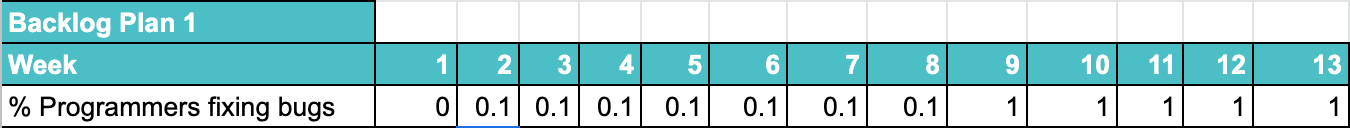
\includegraphics[scale=0.57]{backlog-1-step-1.png}    
    \caption{Programmers fixing bugs}
\end{figure}

\noindent
From week 9 onwards is all hands on deck kind of situation 
and all developers will only work fixing defects. \newline

\noindent
The next step is to figure out how many bugs are fix each week, taking into 
consideration the amount of developers that are available, in description it 
tell us that we cound with 10 programmers which they 
can fix 2 TR per week.\newline

\pagebreak

\noindent
We calculate this in Figure 6, by multiplying the percentage of developers that
are working each week, by the total amount of developers (\textbf{10}), and we multiply that by 
the amount of TR that they are able to fix by week (\textbf{2}).\newline

\begin{figure}[!htb]
    \centering
    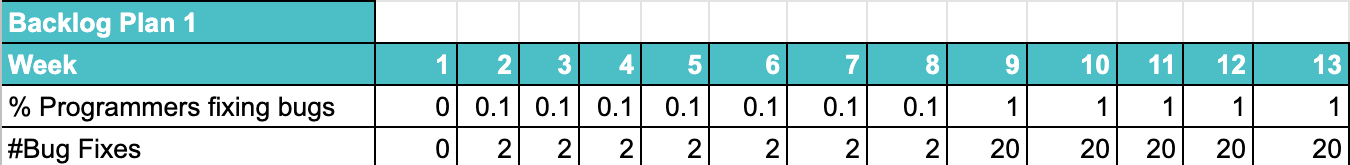
\includegraphics[scale=0.57]{backlog-1-step-2.png}    
    \caption{Bug Fixes}
\end{figure}

\noindent
The last step is see how many bugs are able to get fixed by the end of each,
we do that by taking the amount of defects from the week, subtracting the 
number of defects that the team is able to fix and we add the number of defects 
from the previous week. \newline

\begin{figure}[!htb]
    \centering
    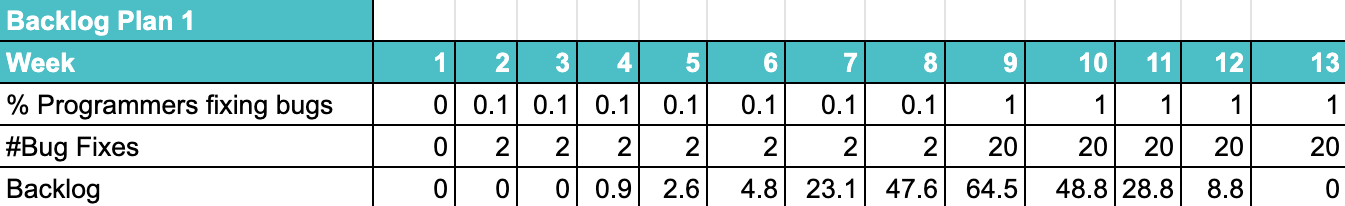
\includegraphics[scale=0.57]{backlog-1-step-3.png}    
    \caption{Backlog}
\end{figure}

\noindent
If for some reason the team is able to fix more defects that the one that 
arrive, we flat the value to 0 because we can't have negative defects fixed

\subsection{Conclusion}
With this backlog approach we are able to clear the backlog in \textbf{13 weeks}.
